\subsection*{2.3 Non Linear Function }

\vspace{0.5em}

\setcounter{questionnum}{0}

\noindent\markforreview
\vspace{1em}

The quadratic function $h$ is defined as $h(x) = 2(x - 4)^2 - 32$.  
In the $xy$-plane, the graph of $y = h(x)$ intersects the $x$-axis at the points $(0, 0)$ and $(t, 0)$, where $t$ is a constant.  
What is the value of $t$?

\vspace{0.75em}

\choicebox{A}{$1$}
\choicebox{B}{$2$}
\choicebox{C}{$4$}
\choicebox{D}{$8$}

\vspace{2em}

\noindent\markforreview
\vspace{1em}

The function $f$ is defined by $f(x) = (-8)(2)^x + 22$.  
What is the $y$-intercept of the graph of $y = f(x)$ in the $xy$-plane?

\vspace{0.75em}

\choicebox{A}{$(0, 14)$}
\choicebox{B}{$(0, 2)$}
\choicebox{C}{$(0, 22)$}
\choicebox{D}{$(0, -8)$}

\vspace{2em}
\newpage
\noindent\markforreview
\vspace{1em}

The function $f$ is defined by $f(x) = 9,\!000(0.66)^x$.  
The function models the number of advertisements a company sent to its clients each year, where $x$ is the number of years since 1997, and $0 \leq x \leq 5$.  
If $y = f(x)$ is graphed in the $xy$-plane, which of the following is the best interpretation of the $y$-intercept?

\vspace{0.75em}

\choicebox{A}{The minimum estimated number of advertisements the company sent to its clients during the 5 years was 1,708.}
\choicebox{B}{The minimum estimated number of advertisements the company sent to its clients during the 5 years was 9,000.}
\choicebox{C}{The estimated number of advertisements the company sent to its clients in 1997 was 1,708.}
\choicebox{D}{The estimated number of advertisements the company sent to its clients in 1997 was 9,000.}

\vspace{2em}

\noindent\markforreview
\vspace{1em}

The first term of a sequence is $9$. Each term after the first is $4$ times the preceding term.  
If $w$ represents the $n$th term of the sequence, which equation gives $w$ in terms of $n$?

\vspace{0.75em}

\choicebox{A}{$w = 4(9^n)$}
\choicebox{B}{$w = 4(9^{n - 1})$}
\choicebox{C}{$w = 9(4^n)$}
\choicebox{D}{$w = 9(4^{n - 1})$}

\vspace{2em}
\newpage
\noindent\markforreview
\vspace{1em}

Function $f$ is defined by $f(x) = -a^x + b$, where $a$ and $b$ are constants.  
In the $xy$-plane, the graph of $y = f(x) - 12$ has a $y$-intercept at $(0, -\frac{75}{7})$.  
The product of $a$ and $b$ is $\frac{320}{7}$. What is the value of $a$?

\vspace{2em}

\noindent\markforreview
\vspace{1em}

A machine launches a softball from ground level.  
The softball reaches a maximum height of $51.84$ meters above the ground at $1.8$ seconds and hits the ground at $3.6$ seconds.  
Which equation represents the height above ground $h$, in meters, of the softball $t$ seconds after it is launched?

\vspace{0.75em}

\choicebox{A}{$h = -t^2 + 3.6$}
\choicebox{B}{$h = -t^2 + 51.84$}
\choicebox{C}{$h = -16(t - 1.8)^2 - 3.6$}
\choicebox{D}{$h = -16(t - 1.8)^2 + 51.84$}

\vspace{2em}

\noindent\markforreview
\vspace{1em}

The function $f$ is defined by $f(x) = a^x + b$, where $a$ and $b$ are constants.  
In the $xy$-plane, the graph of $y = f(x)$ has an $x$-intercept at $(2, 0)$ and a $y$-intercept at $(0, -323)$.  
What is the value of $b$?

\vspace{2em}
\newpage
\noindent\markforreview
\vspace{1em}

The revenue $f(x)$, in dollars, that a company receives from sales of a product is given by the function  
$f(x) = -500x^2 + 25,\!000x$, where $x$ is the unit price of the product in dollars.  
The graph of $y = f(x)$ intersects the $x$-axis at $0$ and $a$.  
What does $a$ represent?

\vspace{0.75em}

\choicebox{A}{The revenue, in dollars, when the unit price of the product is \$0}
\choicebox{B}{The unit price, in dollars, of the product that will result in maximum revenue}
\choicebox{C}{The unit price, in dollars, of the product that will result in a revenue of \$0}
\choicebox{D}{The maximum revenue, in dollars, that the company can make}

\vspace{2em}

\noindent\markforreview
\vspace{1em}

\textbf{Growth of a Culture of Bacteria}  
\begin{center}
\begin{tabular}{|c|c|}
\hline
Day & Number of bacteria per milliliter at end of day \\
\hline
1 & $2.5 \times 10^5$ \\
2 & $5.0 \times 10^5$ \\
3 & $1.0 \times 10^6$ \\
\hline
\end{tabular}
\end{center}

A culture of bacteria is growing at an exponential rate, as shown in the table above.  
At this rate, on which day would the number of bacteria per milliliter reach $5.12 \times 10^8$?

\vspace{0.75em}

\choicebox{A}{Day 5}
\choicebox{B}{Day 9}
\choicebox{C}{Day 11}
\choicebox{D}{Day 12}

\vspace{2em}
\newpage
\noindent\markforreview
\vspace{1em}

The function $f(x) = ax^2 + 4x + c$ is a quadratic function, where $a$ and $c$ are constants.  
The graph of $y = f(x)$ in the $xy$-plane is a parabola that opens upward and has a vertex at point $(h, k)$.  
If $k < 0$ and $f(-9) = f(3)$, which of the following must be true?

\begin{itemize}
\item[I.] $c < 0$
\item[II.] $a \geq 1$
\end{itemize}

\vspace{0.75em}

\choicebox{A}{I only}
\choicebox{B}{II only}
\choicebox{C}{I and II}
\choicebox{D}{Neither I nor II}

\vspace{2em}


\noindent\markforreview
\vspace{1em}

The function $f(x) = 4x^2 + 64x + 262$ is defined, and $g(x) = f(x + 5)$.  
For what value of $x$ does $g(x)$ reach its minimum?

\vspace{0.75em}

\choicebox{A}{$-13$}
\choicebox{B}{$-8$}
\choicebox{C}{$-5$}
\choicebox{D}{$-3$}


\newpage

\noindent\markforreview
\vspace{1em}

The function $f(x) = (x - 6)(x - 2)(x + 6)$ is defined.  
In the $xy$-plane, the graph of $y = g(x)$ is the result of translating the graph of $y = f(x)$ up 4 units.  
What is the value of $g(0)$?

\vspace{2em}

\noindent\markforreview
\vspace{1em}

A quadratic function models a projectile’s height, in meters, above the ground in terms of the time, in seconds, after it was launched.  
The model estimates that the projectile was launched from an initial height of $7$ meters above the ground and reached a maximum height of $51.1$ meters above the ground $3$ seconds after the launch.  
How many seconds after the launch does the model estimate that the projectile will return to a height of $7$ meters?

\vspace{0.75em}

\choicebox{A}{$3$}
\choicebox{B}{$6$}
\choicebox{C}{$7$}
\choicebox{D}{$9$}

\vspace{2em}

\noindent\markforreview
\vspace{1em}

Given $y = x^2 - 14x + 22$,  
for what value of $x$ does the value of $y$ reach its minimum?

\vspace{3em}

\noindent\markforreview
\vspace{1em}

Function $f$ is defined by $f(x) = -a^x + b$, where $a$ and $b$ are constants.  
In the $xy$-plane, the graph of $y = f(x) - 15$ has a $y$-intercept at $\left(0, -\frac{99}{7}\right)$.  
The product of $a$ and $b$ is $\frac{65}{7}$. What is the value of $a$?

\newpage

\noindent\markforreview
\vspace{1em}

The function $f(x) = (x - 14)(x + 19)$ is defined.  
For what value of $x$ does $f(x)$ reach its minimum?

\vspace{0.75em}

\choicebox{A}{$-266$}
\choicebox{B}{$-19$}
\choicebox{C}{$-\frac{33}{2}$}
\choicebox{D}{$-\frac{5}{2}$}

\vspace{2em}

\noindent\markforreview
\vspace{1em}

A model estimates that from 2015 to 2020, the number of squirrels in a population increased by $150\%$ of the previous year's value.  
If at the end of 2016, there were $180$ squirrels, which equation represents this model, where $n$ is the estimated number of squirrels $t$ years after 2015 and $t \leq 5$?

\vspace{0.75em}

\choicebox{A}{$n = 72(1.5)^t$}
\choicebox{B}{$n = 72(2.5)^t$}
\choicebox{C}{$n = 180(1.5)^t$}
\choicebox{D}{$n = 180(2.5)^t$}

\vspace{2em}
\newpage
\noindent\markforreview
\vspace{1em}

The function $f(x) = |59 - 2x|$ is defined.  
For which of the following values of $k$ does $f(k) = 3k$?

\vspace{0.75em}

\choicebox{A}{$\frac{59}{5}$}
\choicebox{B}{$\frac{59}{2}$}
\choicebox{C}{$\frac{177}{5}$}
\choicebox{D}{$59$}

\vspace{2em}

\noindent\markforreview
\vspace{1em}

The population $P$ of a certain city $y$ years after the last census is modeled by the equation  
$P = P_0(1 + r)^y$, where $r$ is a constant and $P_0$ is the population when $y = 0$.  
If the population decreases each year by a fixed percent, which of the following must be true?

\vspace{0.75em}

\choicebox{A}{$r < -1$}
\choicebox{B}{$-1 < r < 0$}
\choicebox{C}{$0 < r < 1$}
\choicebox{D}{$r > 1$}

\vspace{2em}
\newpage
\noindent\markforreview
\vspace{1em}

The function $f(x) = 5,\!470(0.64)^{\frac{x}{12}}$ gives the value, in dollars, of a certain piece of equipment after $x$ months of use.  
If the value decreases each year by $p\%$, what is the value of $p$?

\vspace{0.75em}

\choicebox{A}{$4$}
\choicebox{B}{$5$}
\choicebox{C}{$36$}
\choicebox{D}{$64$}

\vspace{2em}

\noindent\markforreview
\vspace{1em}

The function $f(x) = \frac{1}{9}(x - 7)^2 + 3$ gives a metal ball's height above the ground $f(x)$, in inches, $x$ seconds after it started moving, where $0 \leq x \leq 10$.  
What is the best interpretation of the vertex of the graph $y = f(x)$?

\vspace{0.75em}

\choicebox{A}{The metal ball's minimum height was 3 inches above the ground.}
\choicebox{B}{The metal ball's minimum height was 7 inches above the ground.}
\choicebox{C}{The metal ball’s height was 3 inches above the ground when it started moving.}
\choicebox{D}{The metal ball’s height was 7 inches above the ground when it started moving.}

\vspace{2em}
\newpage
\noindent\markforreview
\vspace{1em}

The function $f(t) = 8,\!000(0.65)^t$ models the number of coupons a company sent to customers at the end of each year, where $t$ is the number of years since the end of 1998 and $0 \leq t \leq 5$.  
What is the best interpretation of the $y$-intercept of the graph of $y = f(t)$?

\vspace{0.75em}

\choicebox{A}{The minimum estimated number of coupons the company sent to their customers during the 5 years was 1,428.}
\choicebox{B}{The minimum estimated number of coupons the company sent to their customers during the 5 years was 8,000.}
\choicebox{C}{The estimated number of coupons the company sent to their customers at the end of 1998 was 1,428.}
\choicebox{D}{The estimated number of coupons the company sent to their customers at the end of 1998 was 8,000.}

\vspace{2em}

\noindent\markforreview
\vspace{1em}

In the $xy$-plane, a parabola has vertex $(9, -14)$ and intersects the $x$-axis at two points.  
If the equation of the parabola is written as $y = ax^2 + bx + c$, what could be the value of $a + b + c$?

\vspace{0.75em}

\choicebox{A}{$-23$}
\choicebox{B}{$-19$}
\choicebox{C}{$-14$}
\choicebox{D}{$-12$}


\newpage
\noindent\markforreview
\vspace{1em}

\textbf{The table below gives selected values of a polynomial function $p$:}

\begin{center}
\begin{tabular}{|c|c|}
\hline
$x$ & $p(x)$ \\
\hline
$-2$ & $5$ \\
$-1$ & $0$ \\
$0$ & $-3$ \\
$1$ & $-1$ \\
$2$ & $0$ \\
\hline
\end{tabular}
\end{center}

Based on the values in the table, which of the following must be a factor of $p$?

\vspace{0.75em}

\choicebox{A}{$(x - 3)$}
\choicebox{B}{$(x + 3)$}
\choicebox{C}{$(x - 1)(x + 2)$}
\choicebox{D}{$(x + 1)(x - 2)$}

\vspace{1.3em}

\noindent\markforreview
\vspace{1em}

When the quadratic function $f$ is graphed in the $xy$-plane, where $y = f(x)$, its vertex is $(-3, 6)$.  
One of the $x$-intercepts of this graph is $\left(-\frac{17}{4}, 0\right)$.  
What is the other $x$-intercept?

\vspace{0.75em}

\choicebox{A}{$\left(-\frac{29}{4}, 0\right)$}
\choicebox{B}{$\left(-\frac{7}{4}, 0\right)$}
\choicebox{C}{$\left(\frac{5}{4}, 0\right)$}
\choicebox{D}{$\left(\frac{17}{4}, 0\right)$}

\vspace{2em}

\noindent\markforreview
\vspace{1em}

The function $f(x) = (x + 3)(x + 1)$ is graphed in the $xy$-plane.  
Which of the following intervals contains the $x$-coordinate of the vertex of the graph of $f$?

\vspace{0.75em}

\choicebox{A}{$-4 < x < -3$}
\choicebox{B}{$-3 < x < 1$}
\choicebox{C}{$1 < x < 3$}
\choicebox{D}{$3 < x < 4$}

\vspace{2em}

\noindent\markforreview
\vspace{1em}

A landscaper is designing a rectangular garden. The length is 5 feet longer than the width.  
If the area is $104$ square feet, what will be the length in feet?

\vspace{5em}

\noindent\markforreview
\vspace{1em}

$P(t) = 290(1.04)^{\frac{4}{6}t}$ models the population, in thousands, of a certain city $t$ years after 2005.  
The population increases by $n\%$ every 18 months. What is the value of $n$?

\vspace{0.75em}

\choicebox{A}{$0.38$}
\choicebox{B}{$1.04$}
\choicebox{C}{$4$}
\choicebox{D}{$6$}

\newpage

\noindent\markforreview
\vspace{1em}

For the function $f$, $f(0) = 86$, and for each increase in $x$ by $1$, $f(x)$ decreases by $80\%$.  
What is the value of $f(2)$?

\vspace{2em}

\noindent\markforreview
\vspace{1em}

$M = 1,\!800(1.02)^t$ models gym members, M, of a gym $t$ years after opening.  
Which equation models the number of members $q$ quarter-years after opening?

\vspace{0.75em}

\choicebox{A}{$M = 1,\!800(1.02)^{q/4}$}
\choicebox{B}{$M = 1,\!800(1.02)^{4q}$}
\choicebox{C}{$M = 1,\!800(1.005)^{4q}$}
\choicebox{D}{$M = 1,\!800(1.082)^q$}

\vspace{2em}

\noindent\markforreview
\vspace{1em}
The functions f and g are defined by the given equation, where $ x \geq0$. Which function shows a maximum value as a constant or coefficient for $x \geq 0$?

\begin{itemize}
    \item[I]  $f(x) = 33(0.4)^{x + 3}$ 
 
\item[II] $g(x) = 33(0.16)(0.4)^{x - 2}$. 
\end{itemize}

\vspace{0.75em}

\choicebox{A}{I only}
\choicebox{B}{II only}
\choicebox{C}{I and II}
\choicebox{D}{Neither I nor II}

\newpage
\noindent\markforreview
\vspace{1em}

Square $P$ has a side length of $x$ inches. Square $Q$ has a perimeter that is  $176$ inches greater than the perimeter of square $P$.  
The function $f$ gives the area of square $Q$, in inches. Which of the following defines $f$?

\vspace{0.75em}

\choicebox{A}{$f(x) = (x + 44)^2$}
\choicebox{B}{$f(x) = (x + 176)^2$}
\choicebox{C}{$f(x) = (176x + 44)^2$}
\choicebox{D}{$f(x) = (176x + 176)^2$}

\vspace{2em}

\noindent\markforreview
\vspace{1em}

The surface area of a cube is $6\left(\frac{a}{4}\right)^2$, where $a$ is a positive constant.  
Which of the following gives the perimeter of one face of the cube?

\vspace{0.75em}

\choicebox{A}{$\frac{a}{4}$}
\choicebox{B}{$a$}
\choicebox{C}{$4a$}
\choicebox{D}{$6a$}

\newpage

\noindent\markforreview
\vspace{1em}

The function $h(x) = a^x + b$, where a and b are positive constants, passes through $(0, 10)$ and $(-2, \frac{325}{36})$.  
What is the value of $ab$?

\vspace{0.75em}

\choicebox{A}{$\frac{1}{4}$}
\choicebox{B}{$\frac{1}{2}$}
\choicebox{C}{$54$}
\choicebox{D}{$60$}

\vspace{2em}

\noindent\markforreview
\vspace{1em}

\textbf{Table:}
\begin{center}
\begin{tabular}{|c|c|}
\hline
$x$ & $y$ \\
\hline
$21$ & $-8$ \\
$23$ & $8$ \\
$25$ & $-8$ \\
\hline
\end{tabular}
\end{center}

The table shows three values of x and their corresponding values of y. Given $y = f(x) + 4$, and $f$ is quadratic function, what is the $y$-coordinate of the $y$-intercept of $y = f(x)$?

\newpage

\noindent\markforreview
\vspace{1em}

A quadratic function models the height, in feet, of an object above the ground in terms of the time, in seconds, after the object is launched off an elevated surface. The model indicates the object has an initial height of 10 feet above the ground and reaches its maximum height of 1,034 feet above the ground 8 seconds after being launched. Based on the model, what is the height, in feet, of the object above the ground 10 seconds after being launched?

\vspace{0.75em}

\choicebox{A}{$234$}
\choicebox{B}{$778$}
\choicebox{C}{$970$}
\choicebox{D}{$1,\!014$}

\vspace{2em}

\noindent\markforreview
\vspace{1em}

Function $f$ is defined by $f(x) = (x + 6)(x + 5)(x + 1)$.  
Function $g$ is defined by $g(x) = f(x - 1)$.  
The graph of $y = g(x)$ in the $xy$-plane has $x$-intercepts at $(a, 0)$, $(b, 0)$, and $(c, 0)$, where $a$, $b$, and $c$ are distinct constants.  
What is the value of $a + b + c$?

\vspace{0.75em}

\choicebox{A}{$-15$}
\choicebox{B}{$-9$}
\choicebox{C}{$11$}
\choicebox{D}{$15$}

\newpage

\noindent\markforreview
\vspace{1em}

The total distance $d$, in meters, traveled by an object moving in a straight line can be modeled by a quadratic function that is defined in terms of $t$, where $t$ is the time in seconds. At a time of 10.0 seconds, the total distance traveled by the object is 50.0 meters, and at a time of 20.0 seconds, the total distance traveled by the object is 200.0 meters. If the object was at a distance of 0 meters when $t = 0$, then what is the total distance traveled, in meters, by the object after 30.0 seconds?

\vspace{2em}

\noindent\markforreview
\vspace{1em}

$f(x) = 4x^2 - 50x + 126$  
The given equation defines the function $f$.  
For what value of $x$ does $f(x)$ reach its minimum?

\vspace{2em}

\noindent\markforreview
\vspace{1em}

$h(x) = x^3 + ax^2 + bx + c$

The function $h$ is defined above, where $a$, $b$, and $c$ are integer constants.  
If the zeros of the function are $-5$, $6$, and $7$, what is the value of $c$?

\vspace{2em}

\noindent\markforreview
\vspace{1em}
\[f(x) = 9(4)^x\]


The function $f$ is defined by the given equation.  
If $g(x) = f(x + 2)$, which of the following equations defines the function $g$?

\vspace{0.75em}

\choicebox{A}{$g(x) = 18(4)^x$}
\choicebox{B}{$g(x) = 144(4)^x$}
\choicebox{C}{$g(x) = 18(8)^x$}
\choicebox{D}{$g(x) = 81(16)^x$}

\vspace{2em}


\newpage
\noindent\markforreview
\vspace{1em}

\[f(x) = (x + 7)^2 + 4\]


The function $f$ is defined by the given equation.  
For what value of $x$ does $f(x)$ reach its minimum?

\vspace{2em}
\noindent\markforreview
\vspace{1em}

Kao measured the temperature of a cup of hot chocolate placed in a room with a constant temperature of 70 degrees Fahrenheit (°F).  
The temperature of the hot chocolate was $185^\circ$F at 6:00 p.m. when it started cooling.  
The temperature of the hot chocolate was $156^\circ$F at 6:05 p.m. and $135^\circ$F at 6:10 p.m.  
The hot chocolate’s temperature continued to decrease.  
Of the following functions, which best models the temperature $T(m)$, in degrees Fahrenheit, of Kao’s hot chocolate $m$ minutes after it started cooling?

\vspace{0.75em}

\choicebox{A}{$T(m) = 185(1.25)^m$}  
\choicebox{B}{$T(m) = 185(0.85)^m$}  
\choicebox{C}{$T(m) = (185 - 70)(0.75)^{\frac{m}{5}}$}  
\choicebox{D}{$T(m) = 70 + 115(0.75)^{\frac{m}{5}}$}



\newpage

\noindent\markforreview
\vspace{1em}


\[p(t) = 90,\!000(1.06)^t\]


The given function $p$ models the population of Lowell $t$ years after a census.  
Which of the following functions best models the population of Lowell $m$ months after the census?

\vspace{0.75em}

\choicebox{A}{$r(m) = \frac{90,\!000}{12}(1.06)^m$}
\choicebox{B}{$r(m) = 90,\!000\left(\frac{1.06}{12}\right)^m$}
\choicebox{C}{$r(m) = 90,\!000\left(\frac{1.06}{12}\right)^{\frac{m}{12}}$}
\choicebox{D}{$r(m) = 90,\!000(1.06)^{\frac{m}{12}}$}

\vspace{2em}

\noindent\markforreview
\vspace{1em}

The population of a town is currently $50,\!000$, and the population is estimated to increase each year by $3\%$ from the previous year.  
Which of the following equations can be used to estimate the number of years $t$ it will take for the population of the town to reach $60,\!000$?

\vspace{0.75em}

\choicebox{A}{$50,\!000 = 60,\!000(0.03)^t$}
\choicebox{B}{$50,\!000 = 60,\!000(3)^t$}
\choicebox{C}{$60,\!000 = 50,\!000(0.03)^t$}
\choicebox{D}{$60,\!000 = 50,\!000(1.03)^t$}
\newpage

\noindent\markforreview
\vspace{1em}

For the exponential function $f$, the value of $f(1)$ is $k$, where $k$ is a constant.  
Which of the following equivalent forms of the function $f$ shows the value of $k$ as the coefficient or the base?

\vspace{0.75em}

\choicebox{A}{$f(x) = 50(2)^{x+1}$}
\choicebox{B}{$f(x) = 80(2)^x$}
\choicebox{C}{$f(x) = 128(2)^{x-1}$}
\choicebox{D}{$f(x) = 205(2)^{x-2}$}

\vspace{2em}

\noindent\markforreview
\vspace{1em}

\[h(x) = -16x^2 + 100x + 10\]


The quadratic function above models the height above the ground $h$, in feet, of a projectile $x$ seconds after it had been launched vertically.  
If $y = h(x)$ is graphed in the $xy$-plane, which of the following represents the real-life meaning of the positive $x$-intercept of the graph?

\vspace{0.75em}

\choicebox{A}{The initial height of the projectile}
\choicebox{B}{The maximum height of the projectile}
\choicebox{C}{The time at which the projectile reaches its maximum height}
\choicebox{D}{The time at which the projectile hits the ground}

\newpage

\noindent\markforreview
\vspace{1em}

\begin{center}
\begin{tabular}{|c|c|}
\hline
$x$ & $f(x)$ \\
\hline
$1$ & $a$ \\
$2$ & $a^5$ \\
$3$ & $a^9$ \\
\hline
\end{tabular}
\end{center}

For the exponential function $f$, the table above shows several values of $x$ and their corresponding values of $f(x)$,  
where $a$ is a constant greater than $1$. If $k$ is a constant and $f(k) = a^{29}$, what is the value of $k$?


\vspace{2em}

\noindent\markforreview

\begin{center}
    

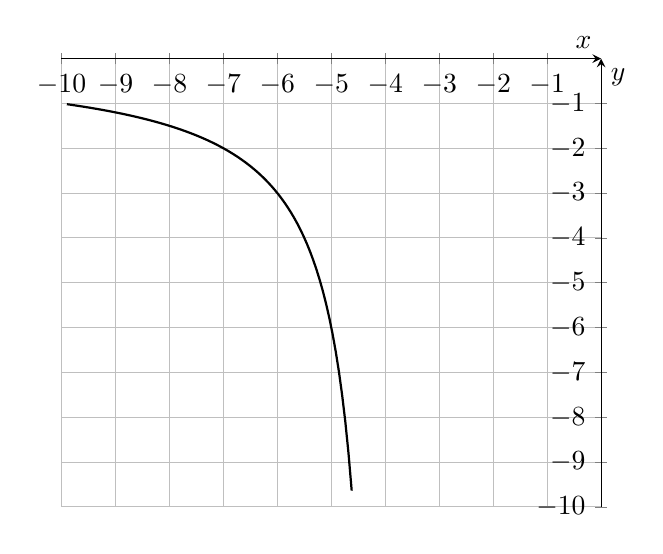
\begin{tikzpicture}
\begin{axis}[
    axis lines=center,
    xlabel=$x$, ylabel=$y$,
    xmin=-10, xmax=0,
    ymin=-10, ymax=0,
    xtick={-10,-9,...,0},
    ytick={-10,-9,...,0},
    samples=200,
    grid=major,
    domain=-9.9:1.9,
    restrict y to domain=-10:10
]
\addplot[thick, black] {6 / (x + 4)};
\end{axis}
\end{tikzpicture}

\end{center}

The rational function $f$ is defined by an equation in the form $f(x) = \dfrac{a}{x + b}$, where $a$ and $b$ are constants.  
The partial graph of $y = f(x)$ is shown.  
If $g(x) = f(x + 4)$, which equation could define function $g$?

\vspace{0.40em}

\choicebox{A}{$g(x) = \dfrac{6}{x}$}
\choicebox{B}{$g(x) = \dfrac{6}{x + 4}$}
\choicebox{C}{$g(x) = \dfrac{6}{x + 8}$}
\choicebox{D}{$g(x) = \dfrac{6(x - 4)}{x + 4}$}

\vspace{2em}

\noindent\markforreview
\vspace{1em}

$f(x) = (x - 10)(x + 13)$

The function $f$ is defined by the given equation.  
For what value of $x$ does $f(x)$ reach its minimum?

\vspace{0.75em}

\choicebox{A}{$-130$}
\choicebox{B}{$-13$}
\choicebox{C}{$-\dfrac{23}{2}$}
\choicebox{D}{$-\dfrac{3}{2}$}

\vspace{2em}

\noindent\markforreview
\vspace{1em}

For the function $q$, the value of $q(x)$ decreases by $45\%$ for every increase in the value of $x$ by $1$.  
If $q(0) = 14$, which equation defines $q$?

\vspace{0.75em}

\choicebox{A}{$q(x) = 0.55(14)^x$}
\choicebox{B}{$q(x) = 1.45(14)^x$}
\choicebox{C}{$q(x) = 14(0.55)^x$}
\choicebox{D}{$q(x) = 14(1.45)^x$}

\newpage
\noindent\markforreview
\vspace{1em}

Two variables, $x$ and $y$, are related such that for each increase of $1$ in the value of $x$, the value of $y$ increases by a factor of $4$.  
When $x = 0$, $y = 200$. Which equation represents this relationship?

\vspace{0.75em}

\choicebox{A}{$y = 4(x)^{200}$}
\choicebox{B}{$y = 4(200)^x$}
\choicebox{C}{$y = 200(4)^x$}
\choicebox{D}{$y = 200(4x)$}

\vspace{2em}

\noindent\markforreview
\vspace{1em}

What is the minimum value of the function $f$ defined by $f(x) = (x - 2)^2 - 4$?

\vspace{0.75em}

\choicebox{A}{$-4$}
\choicebox{B}{$-2$}
\choicebox{C}{$2$}
\choicebox{D}{$4$}

\newpage

\noindent\markforreview
\vspace{1em}

Let the function $p$ be defined as $p(x) = \dfrac{(x - c)^2 + 160}{2c}$, where $c$ is a constant.  
If $p(c) = 10$, what is the value of $p(12)$?

\vspace{0.75em}

\choicebox{A}{$10.00$}
\choicebox{B}{$10.25$}
\choicebox{C}{$10.75$}
\choicebox{D}{$11.00$}






























